\documentclass[a4paper, 14pt]{extarticle}

% Поля
%--------------------------------------
\usepackage{geometry}
\geometry{a4paper,tmargin=2cm,bmargin=2cm,lmargin=3cm,rmargin=1cm}
%--------------------------------------


%Russian-specific packages
%--------------------------------------
\usepackage[T2A]{fontenc}
\usepackage[utf8]{inputenc} 
\usepackage[english, main=russian]{babel}
%--------------------------------------

\usepackage{textcomp}

% Красная строка
%--------------------------------------
\usepackage{indentfirst}               
%--------------------------------------             


%Graphics
%--------------------------------------
\usepackage{graphicx}
\graphicspath{ {./images/} }
\usepackage{wrapfig}
%--------------------------------------

% Полуторный интервал
%--------------------------------------
\linespread{1.3}                    
%--------------------------------------

%Выравнивание и переносы
%--------------------------------------
% Избавляемся от переполнений
\sloppy
% Запрещаем разрыв страницы после первой строки абзаца
\clubpenalty=10000
% Запрещаем разрыв страницы после последней строки абзаца
\widowpenalty=10000
%--------------------------------------

%Списки
\usepackage{enumitem}

%Подписи
\usepackage{caption} 

%Гиперссылки
\usepackage{hyperref}

\hypersetup {
	unicode=true
}

%Рисунки
%--------------------------------------
\DeclareCaptionLabelSeparator*{emdash}{~--- }
\captionsetup[figure]{labelsep=emdash,font=onehalfspacing,position=bottom}
%--------------------------------------

\usepackage{tempora}

%Листинги
%--------------------------------------
\usepackage{listings}
\lstset{
  basicstyle=\ttfamily\footnotesize, 
  %basicstyle=\footnotesize\AnkaCoder,        % the size of the fonts that are used for the code
  breakatwhitespace=false,         % sets if automatic breaks shoulbd only happen at whitespace
  breaklines=true,                 % sets automatic line breaking
  captionpos=t,                    % sets the caption-position to bottom
  inputencoding=utf8,
  frame=single,                    % adds a frame around the code
  keepspaces=true,                 % keeps spaces in text, useful for keeping indentation of code (possibly needs columns=flexible)
  keywordstyle=\bf,       % keyword style
  numbers=left,                    % where to put the line-numbers; possible values are (none, left, right)
  numbersep=5pt,                   % how far the line-numbers are from the code
  xleftmargin=25pt,
  xrightmargin=25pt,
  showspaces=false,                % show spaces everywhere adding particular underscores; it overrides 'showstringspaces'
  showstringspaces=false,          % underline spaces within strings only
  showtabs=false,                  % show tabs within strings adding particular underscores
  stepnumber=1,                    % the step between two line-numbers. If it's 1, each line will be numbered
  tabsize=2,                       % sets default tabsize to 8 spaces
  title=\lstname                   % show the filename of files included with \lstinputlisting; also try caption instead of title
}
%--------------------------------------

%%% Математические пакеты %%%
%--------------------------------------
\usepackage{amsthm,amsfonts,amsmath,amssymb,amscd}  % Математические дополнения от AMS
\usepackage{mathtools}                              % Добавляет окружение multlined
\usepackage[perpage]{footmisc}
%--------------------------------------

%--------------------------------------
%			НАЧАЛО ДОКУМЕНТА
%--------------------------------------

\begin{document}

%--------------------------------------
%			ТИТУЛЬНЫЙ ЛИСТ
%--------------------------------------
\begin{titlepage}
\thispagestyle{empty}
\newpage


%Шапка титульного листа
%--------------------------------------
\vspace*{-60pt}
\hspace{-65pt}
\begin{minipage}{0.3\textwidth}
\hspace*{-20pt}\centering

\includegraphics[width=\textwidth]{emblem}
\end{minipage}
\begin{minipage}{0.67\textwidth}\small \textbf{
\vspace*{-0.7ex}
\hspace*{-6pt}\centerline{Министерство науки и высшего образования Российской Федерации}
\vspace*{-0.7ex}
\centerline{Федеральное государственное бюджетное образовательное учреждение }
\vspace*{-0.7ex}
\centerline{высшего образования}
\vspace*{-0.7ex}
\centerline{<<Московский государственный технический университет}
\vspace*{-0.7ex}
\centerline{имени Н.Э. Баумана}
\vspace*{-0.7ex}
\centerline{(национальный исследовательский университет)>>}
\vspace*{-0.7ex}
\centerline{(МГТУ им. Н.Э. Баумана)}}
\end{minipage}
%--------------------------------------

%Полосы
%--------------------------------------
\vspace{-25pt}
\hspace{-35pt}\rule{\textwidth}{2.3pt}

\vspace*{-20.3pt}
\hspace{-35pt}\rule{\textwidth}{0.4pt}
%--------------------------------------

\vspace{1.5ex}
\hspace{-35pt} \noindent \small ФАКУЛЬТЕТ\hspace{80pt} <<Информатика и системы управления>>

\vspace*{-16pt}
\hspace{47pt}\rule{0.83\textwidth}{0.4pt}

\vspace{0.5ex}
\hspace{-35pt} \noindent \small КАФЕДРА\hspace{50pt} <<Теоретическая информатика и компьютерные технологии>>

\vspace*{-16pt}
\hspace{30pt}\rule{0.866\textwidth}{0.4pt}
  
\vspace{11em}

\begin{center}
\Large {\bf Лабораторная работа № 2} \\ 
\large {\bf по курсу <<Языки и методы программирования>>} \\
\large <<Разработка простейшего класса на языке Java>> \\
\Large Вариант 10
\end{center}\normalsize

\vspace{8em}


\begin{flushright}
  {Студент группы ИУ9-21Б Шиятов Н. \hspace*{15pt}\\ 
  \vspace{2ex}
  Преподаватель Посевин Д. П.\hspace*{15pt}}
\end{flushright}

\bigskip

\vfill
 

\begin{center}
\textsl{Москва 2023}
\end{center}
\end{titlepage}
%--------------------------------------
%		КОНЕЦ ТИТУЛЬНОГО ЛИСТА
%--------------------------------------

\renewcommand{\ttdefault}{pcr}

\setlength{\tabcolsep}{3pt}
\newpage
\setcounter{page}{2}

\section{Задание}\label{Sect::task}

Выполнение лабораторной работы заключается в составлении на языке Java одного из
классов, приведённых в таблице. В классе обязательно должны присутствовать конструктор и
метод toString.
Отладку разработанного класса необходимо осуществить в методе main
вспомогательного класса Test. Использование контейнерных классов из стандартной библиотеки
языка Java не разрешается.

№ 10. Класс ломаных линий в двумерном пространстве с операцией вычисления длины ломаной.

\section{Результаты}\label{Sect::res}

Исходный код программы представлен в листингах~\ref{lst:main}--~\ref{lst:polyline}.

Результат запуска представлен на рисунке~\ref{fig:output}.


\begin{figure}[!htb]
\begin{lstlisting}[language=Java,caption={Класс Main},label={lst:main}]
public class Main {
    public Main() {
    }

    public static void main(String[] args) {
        int n = 5;
        Line[] lines = new Line[n];

        for(int i = 0; i < n; ++i) {
            Point PointA = new Point("A", 1.0, 0.0);
            Point PointB = new Point("B", 2.0, 1.0);
            lines[i] = new Line("Line" + i, PointA, PointB);
        }

        Polyline poly = new Polyline("My poplyline", lines);
        System.out.println(poly.getPolylineLength());
    }
}

\end{lstlisting}
\end{figure}

\newpage

\begin{figure}[!htb]
\begin{lstlisting}[language=Java,caption={Класс Point},label={lst:point}]
public class Point {
    private String name;
    private double x;
    private double y;
    private static int PointCounter;

    public Point(String argName) {
        ++PointCounter;
        System.out.println("An object of the Point class has been created");
        this.name = argName;
    }

    public Point(String argName, double argX, double argY) {
        ++PointCounter;
        System.out.println("An object of the Point class has been created");
        this.x = argX;
        this.y = argY;
    }

    public double getXCoord() {
        return this.x;
    }

    public double getYCoord() {
        return this.y;
    }

    public String getName() {
        return this.name;
    }

    public void setCoord(double varX, double varY) {
        this.x = varX;
        this.y = varY;
    }
}
\end{lstlisting}
\end{figure}

\newpage

\begin{figure}[!htb]
\begin{lstlisting}[language=Java,caption={Класс Line},label={lst:line}]
public class Line {
    private String name;
    private double x;
    private double y;
    private static int LineCounter;

    public Line(String argName) {
        ++LineCounter;
        System.out.println("An object of the Line class has been created");
        this.name = argName;
    }

    public Line(String argName, Point argA, Point argB) {
        ++LineCounter;
        System.out.println("An object of the Line class has been created");
        this.x = Math.abs(argA.getXCoord() - argB.getXCoord());
        this.y = Math.abs(argA.getYCoord() - argB.getYCoord());
    }

    public String getName() {
        return this.name;
    }

    public double getXCoord() {
        return this.x;
    }

    public double getYCoord() {
        return this.y;
    }

    public void setCoord(double argX, double argY) {
        this.x = argX;
        this.y = argY;
    }

    public double getLineLength() {
        return Math.pow(Math.pow(this.x, 2.0) + Math.pow(this.y, 2.0), 0.5);
    }
}
\end{lstlisting}
\end{figure}

\newpage

\begin{figure}[!htb]
\begin{lstlisting}[language=Java,caption={Класс Polyline},label={lst:polyline}]
public class Polyline {
    private String name;
    private Line[] linesArr;

    public Polyline(String argName) {
        System.out.println("An object of the Polyline class has been created");
        this.name = argName;
    }

    public Polyline(String argName, Line[] argLines) {
        System.out.println("An object of the Polyline class has been created");
        this.name = argName;
        this.linesArr = argLines;
    }

    public double getPolylineLength() {
        int len = 0;

        for(int i = 0; i < this.linesArr.length; ++i) {
            len = (int)((double)len + this.linesArr[i].getLineLength());
        }

        return (double)len;
    }
}
\end{lstlisting}
\end{figure}


\begin{figure}[!htb]
	\centering
	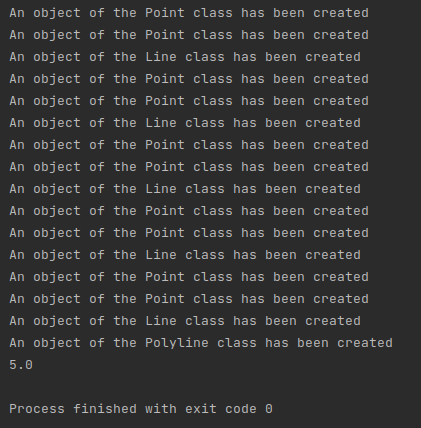
\includegraphics[width=0.8\textwidth]{output.png}
\caption{Результат}
\label{fig:output}
\end{figure}

\end{document}